\documentclass[conference]{IEEEtran}
\usepackage[spanish, es-tabla, activeacute]{babel}
\usepackage[utf8]{inputenc}
\usepackage{amsmath, amssymb}
\usepackage{graphicx}
\usepackage{anysize}
\usepackage{hyperref}
\usepackage{caption}
\usepackage[table]{xcolor}
\usepackage{booktabs}

\usepackage{color}
\newcommand{\todo}{\textcolor{red}{TO DO:}\textcolor{blue}}
\newcommand{\ror}{\emph{Ruby on Rails}}

%\renewcommand{\listtablename}{Índice de tablas}
\renewcommand{\tablename}{Tabla}

\title{ChiVO: Estado actual del Observatorio Virtual de Chile}
\author{
\IEEEauthorblockN{
    Jonathan Antognini \IEEEauthorrefmark{1},
    Mauricio Araya     \IEEEauthorrefmark{1},
    Mauricio Solar     \IEEEauthorrefmark{1} \\
}
\IEEEauthorblockA{
    \IEEEauthorrefmark{1} Universidad Técnica Federico Santa María,Valparaiso, Chile}
}

\begin{document}

\maketitle

\begin{abstract}
This paper presents the challenges, architecture and current status of the
Chilean Virtual Observatory (ChiVO), which is a software infrastructure 
for accessing and processing astronomical data generated in Chile. As ChiVO
is part of the International Virtual Observatory Alliance (IVOA), 
we strictly follow the protocols and standards that this
organization produce. However, there are always open challenges due to the
new observational technologies and local requirements 
that motivates research on every new 
virtual observatory, such as the complex data models and Big Data problems 
that the ALMA Observatory is confronting. 
The current ChiVO prototype includes IVOA compliant services as well as
new solutions designed for ALMA data, all of them using modern software
technologies. 
\end{abstract}
% Maybe agregar que lo esperamos lanzar pronto.

\begin{IEEEkeywords}
ChiVO, Virtual Observatory, Astronomy, IVOA, ALMA.
\end{IEEEkeywords}

\section{Introducción}

Las provilegiadas condiciones atmosféricas hacen de Chile uno de los lugares
más propicios para la realización de investigaciones científicas en astronomía.
Organizaciones astronómicas como el Observatorio Europeo Austral (ESO por sus
siglas en inglés) han elegido asentar sus enormes telescopios en este país para 
llevar a cabo sus descubrimientos\footnote{Acerca de ESO. (s.f.). En
\textit{ESO}. \url{http://www.eso.org/public/chile/about-eso.html}}. 

Existen más de una docena de instalaciones astronómicas de gran envergadura a
lo largo de nuestro territorio nacional \cite{observatorios_chile}, como por
ejemplo ``Atacama Large Milimeter/submilimeter Array'' (ALMA), ``Very Large
Telescope'' (VLT), y en los próximos ``European Extremely Large Telescope''
(E-ELT), con el cual se estima que el 60\% de la observación astronómica
mundial se realice en Chile.  Una de las condiciones que se establecen a nivel
país, es que el 10\% del tiempo de observación pertenece a la comunidad
astronómica chilena. Estos generan datos a gran escala, justificando a nivel
país, el desarrollo de una plataforma astroinformática para su administración y
análisis inteligente.

El Observatorio Virtual (VO por sus siglas en inglés) es una iniciativa
internacional que permite el acceso a archivos astronómicos y centros de datos
a astrónomos y personas comunes a través de Internet. Con la estandarización de
métodos e información es posible estudiar los registros astronómicos sin
requerimientos físicos de instrumentos y locación.

La International Virtual Observatory Alliance (IVOA) fue creada para
``facilitar la coordinación internacional y colaboración necesaria para el
desarrollo y distribución de herramientas, sistemas y estructuras
organizacionales necesarias para permitir la utilización internacional de
archivos astronómicos como un observatorio virtual integrado e 
interoperable\footnote{Traducido de \url{http://www.ivoa.net/about/what-is-ivoa.html}}.
Actualmente, IVOA está compuesta por 19 proyectos\footnote{En el sitio web oficial en la
sección \textbf{What is the IVOA} \textit{``the IVOA now comprises 17 VO
projects''}, pero en \textbf{Members Organizations} aparecen 19 miembros
listados.} de América, Asia, Europa y Oceanía; sus miembros se reunen
dos veces cada año en \textbf{Interoperability Workshops} para entablar
discusiones cara-a-cara y resolver preguntas técnicas.

Actualmente una iniciativa liderada por la UTFSM propone
desarrollar una plataforma astro-informática para la administración y análisis
inteligente de datos a gran escala basados en los estándares de IVOA.  Por lo
anterior, este documento tiene como objetivo:

\begin{itemize}
	\item Dar a conocer la distribución de los VO's en el mundo.
	\item Explicar el concepto de VO.
	\item Explicar la arquitectura a grandes rasgos de un
		VO.
	\item Presentar los primeros pasos para llevar a cabo el
		Chilean Virtual Observatory (ChiVO).
	\item Conclusiones y trabajo a futuro.
\end{itemize}

\section{Arquitectura de ChiVO}

ChiVO es un observatorio virtual en construcción, el cual alojará datos de los
observatorios localizados en Chile, ciñéndose a los estándares de
interoperabilidad de la alianza internacional de observatorios virtuales (IVOA),
y utilizando tecnologías de última generación. Esta sección, detalla el
proceso de diseño realizado para esta iniciativa.

%Que es IVOA?
La misión de IVOA es facilitar la coordinación y colaboración necesaria para
facilitar el acceso global e integrado a los datos recogidos por los
observatorios astronómicos internacionales. Esta organización fue formada en
Junio del 2002 y tiene actualmente 21 miembros activos. Su método de trabajo es
en base a Working Groups, los cuales están a cargo de estabelcer protocolos y
estándares que describen la arquitectura general de un VO \ref{fig:ivoavacio}.
A grandes rasgos, la arquitectura posee tres capas:
\begin{itemize}
    \item Usuarios: astrónomos y científicos en general interesados por los
    datos publicados por los observatorios.
    \item Recursos: observatorios y centros que producen datos astronómicos
    (reales o simulados).
    \item Capa intermedia: esta capa define lo que es un observatorio virtual,
    es decir, de qué manera se comunican los usuarios y recursos usando
    protocolos y estándares para buscar y acceder datos.
\end{itemize}

%Arquitectura de IVOA Vacía
\begin{figure}[ht]
    \centering
    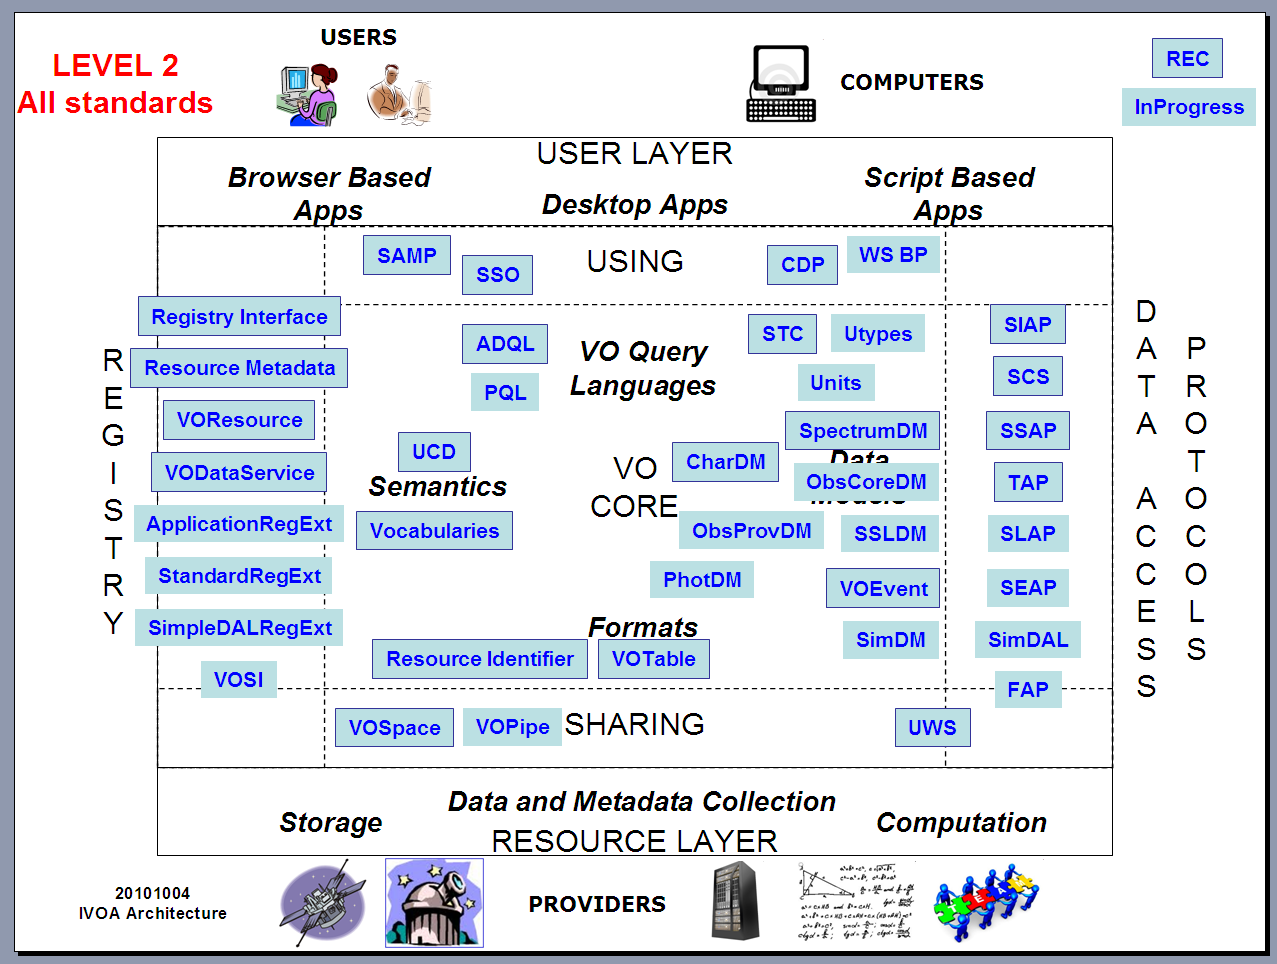
\includegraphics[width=0.45\textwidth]{images/ivoavacio.png}
    \caption{Arquitectura IVOA}
    \label{fig:ivoavacio}
\end{figure}

\subsection{Requerimientos}

Para la creación del ChiVO se identificaron las necesidades actuales de la
comunidad astronómica nacional, las cuales podemos resumir en,

\begin{description}
    \item[Descubrir:] \hfill \\
        Encontrar datos astronómicos de un objeto o instrumento sobre una región
        específica del espacio de alta dimensión, en base a parámetros de los ejes
        espaciales, temporales, espectrales, corrimiento al rojo, polarización, etc,
        ya sea por búsqueda o por exploración.
    \item[Obtener:] \hfill \\
        Enlace a descarga de los datos requeridos en distintos formatos, ya sea en
        el VO o en un servicio externo.
    \item[Comparar:] \hfill \\
        Cruzamiento de información de datos obtenidos entre distintas fuentes de
        información.
\end{description}

En este proceso participó un equipo multidisciplinario (astrónomos, ingenieros,
científicos, expertos en datos de ALMA, etc) y duró aproximadamente 4 meses,
entre que la comunidad astronómica definía bien sus requerimientos y casos de
uso, y entre que el equipo informático contrastaba estos con las normativas
internacionales.

%\textbf{TODO: poner los req?}
%[MA] NO!
%\textbf{Arquitectura IVOA}

\subsection{Arquitectura de ChiVO}

Según las necesidades de los radioastrónomos Chilenos, los requerimientos,
casos de uso y los modelos de datos (compatibles con los estándares de IVOA),
conllevan a la creación de la siguiente arquitectura y modelo de desarrollo
(ver Figura~\ref{fig:chivoarch}).

\begin{figure}[ht]
    \centering
    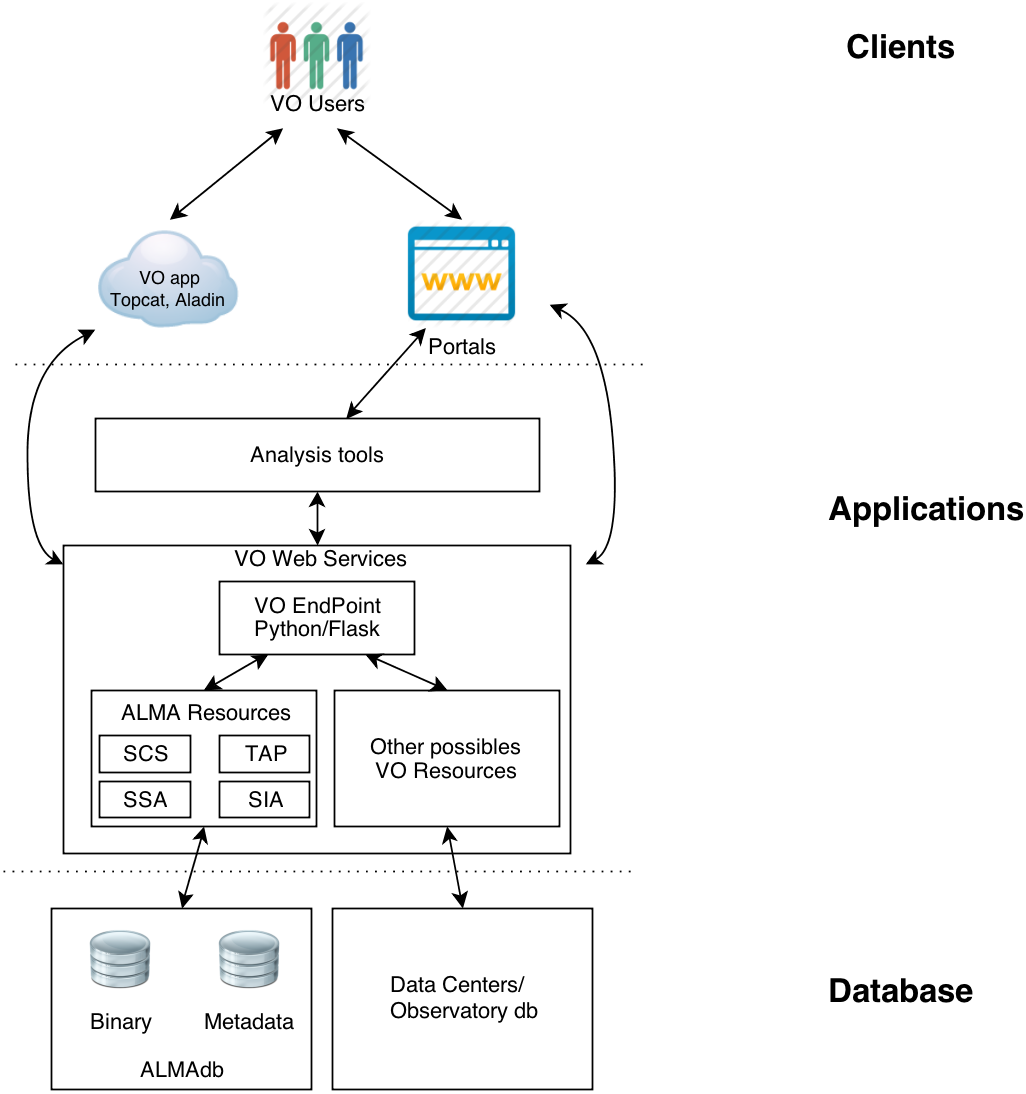
\includegraphics[width=0.45\textwidth]{images/chivo_capas.png}
    \caption{Arquitectura de ChiVO}
    \label{fig:chivoarch}
\end{figure}

\textbf{Capa de abstración: Clientes}

Esta capa representa al usuario final y cómo se facilita la comunicación entre el
usuario y los datos.  En esta capa el usuario realiza consultas a través de los
protocolos de acceso ofrecidos por ChiVO o a través de un formulario avanzado,
utilizando aplicaciones compatibles con VO y su portal web.  Una vez realizada
la consulta, el sistema le retornará al usuario una lista que describe objetos
u observaciones encontrados (metadatos) y podrá acceder a ellos a través de un
enlace de descarga asociado a cada resultado.  Cabe destacar que gracias a la
separación por capas de abstracción se logra la flexibilidad y escalabilidad en
el sistema, para que independientemente de la capa, nuevas aplicaciones puedan
interactuar con ChiVO, así como la adición de nuevas fuentes de información a
parte de ALMA.

Las consultas son recibidas por ChiVO a través de su \emph{endpoint} de datos, que
recibe consultas en \texttt{HTTP}, \texttt{GET} o \texttt{POST}, ante lo cual el
endpoint retorna la lista de resultados en una tabla en el formato XML VOTable 
\cite{ochsenbein2011ivoa}.
Para el caso del portal web, el VOTable es desplegado mostrado al usuario a través
de una herramienta web que permite la manipulación simple y eficiente de VOTables
llamada VOView.

\textbf{Capa de abstracción: Aplicaciones}

En esta capa se encuentran los programas que procesan las consultas entre los
usuarios y los datos.
Cada estándar de IVOA requiere un mínimo de su propia implementación para ser
compatible con el VO, en el caso de estos protocolos de acceso sólo es necesaria la
recepción de consultas HTTP básicas junto a los parámetros de búsqueda requeridos.

El elemento que representa a las herramientas de análisis es fundamental en la
eficiencia de ChiVO, esto es debido a que los datos a analizar por los astrónomos
suelen tener un gran tamaño y es costosa su transferencia, este problema se
resuelve acercando las herramientas de análisis y procesamiento al lugar donde están
almacenados los datos a procesar.

Considerando que en el futuro será necesario ofrecer búsquedas
basadas en otros datos, no sólo provenientes de ALMA, es necesaria cierta
abstracción al momento de implementar esta capa, ya que debe permitir la interacción
nuevas fuentes de información, siempre y cuando se mantenga la compatibilidad
de IVOA.

En esta capa también está en desarrollo un sistema capaz de resolver nombres
(tipo Sesame \cite{sesame} pero para datos de ALMA) y el registro de ChiVO.

\textbf{Capa de abstracción: Datos}

En esta capa se encuentran los recursos que tienen los datos y metadatos.  El
trabajo está asociado a una base de datos relacional para almacenar los
metadatos asociados al modelo de datos recomendado por \emph{IVOA Observation
Core Data Model} \cite{louys2011ivoa}, usando un framework desarrollado por el
VO Alemán DaCHS \cite{dachs}.  Con respecto a rendimiento, nos encontramos en
la sección que consume más recursos, tanto en tiempo de computación (resuelve
las consultas hechas a las base de datos) y además el almacenamiento físico de
los datos.  A modo de verificación momentánea, la actual implementación trabaja
con un conjunto de datos, con un tamaño de 1 TeraByte, los que provienen de la
reducción del ciclo 0 de ALMA.  Debido a esta limitación se propone el esquema
de funcionamiento de la figura \ref{fig:dachs}, en donde pueden haber N
servidores con DaCHS apuntando a M base de datos distribuidas o replicadas.

\begin{figure}[ht]
    \centering
    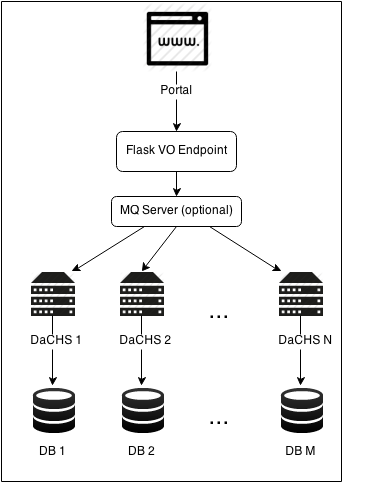
\includegraphics[width=0.45\textwidth]{images/interaccion.png}
    \caption{Configuración de distintas máquinas con base de datos replicadas o distribuidas}
    \label{fig:dachs}
\end{figure}

\subsection{Metadatos de los datos de ALMA}

Para poder construir la base de datos relacional con el modelo de datos ObsCore
fue necesario mapear campos desde el ALMA Science Data Model (ASDM)
\cite{viallefond2009sdm}.  Un ASDM contiene una serie de tablas (XML) con la
metadata de la observación, y en este caso se usaron: \emph{main},
\emph{Source}, \emph{ExecBlock}, \emph{spectralWindow}.

\begin{table}[ht]
    \centering
    \captionof{table}{Campos del ObsCore y origen desde ASDM}
    \begin{tabular}{lr}
        \textbf{Campo ObsCore} & \textbf{ASDM} \\
        dataproduct\_type      & visibility \\
        calib\_level           & 1 \\
        obs\_collection        & ALMA \\
        obs\_id                & [ExecBlock.execBlockUID] \\
        obs\_publisher\_did    & [Cycle ID] \\
        access\_url            & [URL de ChiVO] \\
        access\_format         & application/x-asdm \\
        access\_estsize        & [main.dataSize] \\
        target\_name           & [Source.sourceName] \\
        s\_ra                  & [Source.direction] \\
        s\_dec                 & [Source.direction] \\
        s\_fov                 & [1.2 * lambda / Diametro antena] \\
        s\_region              & circle \\
        s\_resolution          & [1.2*lambda/(ExecBlock.baseRangeMax)] \\
        t\_min                 & [ExecBlock.startTime] \\
        t\_max                 & [ExecBlock.endTime] \\
        t\_exptime             & [main.interval] \\
        t\_resolution          & [mainTable.interval] \\
        em\_min                & [ExecBlock.baseRangeMin] \\
        em\_max                & [ExecBlock.baseRangeMax] \\
        em\_res\_power         & [spectralWindow.resolution] \\
        o\_ucd                 & em.mm \\
        pol\_states            & [Source.stokesParameter[numStokes]] \\
        facility\_name         & ALMA \\
        instrument\_name       & ALMA \\
    \end{tabular}
    \label{table:obsasdm}
\end{table}

En la Tabla \ref{table:obsasdm} se muestra el resultado de la investigación,
a la izquierda se despliegan las columnas de la clase Observation,
la segunda columna indica de donde se obtienen los datos para asignar la los campos
de la primera columna para el caso de los ASDM.

Para poder llenar los campos de la clase Observation es necesario escribir una
rutina capaz de operar sobre las tablas del ASDM (XML).
Actualmente existen múltiples herramientas en el Paquete de Aplicaciones de Software
Comunes de Astronomía (CASA, debido a sus siglas en inglés) \cite{petry2012analysing}.

\subsection{Tecnologías utilizadas}

Para el desarrollo de ChiVO se evaluaron distintas herramientas posibles de las
cuales se concluyó en cada capa:

\textbf{Capa de abstración: Aplicación}

Los framework que se evaluaron para la implementación del endpoint fueron:

\begin{description}
    \item[{\ror}:] \hfill \\
        Framework de desarrollo web ampliamente utilizado el día de hoy,
        se basa en el concepto Modelo-Vista-Controlador (MVC).
        Sin embargo, ésta herramienta no será utilizada debido
        a que muchas funcionalidades no son necesarias para el presente prototipo.
    \item[Python/Flask:] \hfill \\
        Flask es un microframework diseñado especialmente para servicios y
        herramientas web pequeñas.
        La presente solución provee un marco de trabajo para la creación de
        aplicaciones web que puedan ser accedidas mediante distintos métodos
        HTTP.  Existe mucha documentación y comunidad activa que permite
        implementar y solucionar problemas de forma rápida.
\end{description}

\textbf{Capa de abstración: Datos}

Dentro de los \emph{toolkits} de Data Access Layer recomendados por IVOA para
el acceso a datos mediante protocolos: Simple Cone Search (SCS)
\cite{williams2008simple}; Simple Image Access (SIA) \cite{tody2004simple};
Simple Spectral Access (SSA) \cite{tody2008simple}; y Table Access Protocol
(TAP) \cite{dowler2010table} a través de Astronomical Data Query Language (ADQL)
\cite{yasuda2004astronomical} y Universarl Worker Service
\cite{rixon2008universal}, se probaron y verificaron los siguientes:

\begin{description}
    \item[SAADA:] \hfill \\
        Desarrollado por el VO Francés, es una herramienta bastante útil del punto
        de vista del usuario del sistema.
        Posee excelente documentación y un conveniente proceso de instalación.
        Está desarrollado en Java y su correspondiente despliegue se lleva a cabo
        mediante Tomcat.
        Es posible configurar servicios SCS/SIA/SSA/TAP y no es un proyecto
        OpenSource.

    \item[VO-Dance:] \hfill \\
        Desarrollado por el VO Italiano, es una herramienta en Java en su Backend,
        y Python en su Frontend (Framework Django).
        Lo destacable de esta herramienta es que trabaja usando MySQL como motor de
        base de datos principal, y de acuerdo a las últimas noticias relacionadas
        a su desarrollo, podría existir un soporte para PostgreeSQL en el futuro.
        La herramienta no es OpenSource y la documentación es precaria debido
        a que aún está en desarrollo. Compatible con servicios SCS/SIA/SSA/TAP.

    \item[openCADC:] \hfill \\
        Desarrollado por el VO Canadiense, es una herramienta OpenSource escrita en
        Java, utilizada actualmente en el ALMA Science Archive.
        Este toolkit es uno de los más robustos, contiene distintos paquetes con
        servicios a ser utilizados en el webservice, sin embargo posee una
        documentación precaria, lo que es compensado por abierta comunidad de
        desarrollo. Es posible configurar servicios TAP, UWS.

    \item[DaCHS:] \hfill \\
        Desarrollado por el VO Alemán, es una herramienta OpenSource escrita en
        Python.
        Es uno de los toolkits DAL más usados por los VO, ya que posee una amplia
        documentación de instalación y configuración.
        Es posible configurar servicios SCS/SIA/SSA/TAP.
\end{description}

%\vspace{0.5cm}
\begin{table*}[ht]
\centering
\caption{Resumen de los toolkits en tabla comparativa}
\begin{tabular}{lrrrrr}
    {\bf Toolkits} & {\bf Lenguaje} & {\bf OpenSource} & {\bf Documentación} & {\bf Servicios} & {\bf Última actualización}  \\
    SAADA          & Java           & No               & Si                  & SCS/SIA/SSA/TAP & Mayo 2012     \\
    VO-Dance       & Java/Python    & No               & No                  & SCS/SIA/SSA/TAP & Dicimbre 2012 \\
    openCADC       & Java           & Si               & No                  & TAP             & ---           \\
    DaCHS          & Python         & Si               & Si                  & SCS/SIA/SSA/TAP & Junio 2013    \\
\end{tabular}
\label{table:toolkits}
\end{table*}

\textbf{Capa de abstración: Clientes}

Inicialmente la interfaz usuario o frontend poseería solo vistas, por lo que
el desarrollo podía ser en prácticamente cualquier lenguaje o framework, como por
ejemplo PHP, Django o {\ror} Sin embargo con los requerimientos de la
plataforma, especialmente el de capa de usuarios, se decidió escoger un
framework MVC que fuese lo suficientemente ágil y compatible con el resto de
servicios, {\ror}.

\section{Estado de avance}

Para comenzar el desarrollo de ChiVO fue necesario identificar aparte de los
requerimientos y casos de uso, las interacciones que los usuarios realizarán
con el sistema. El diagrama de secuencia de interacción entre el usuario y
ChiVO se puede ver en la figura \ref{fig:secuencia}.
En base a este diagrama, requerimientos y tecnologías utilizadas el estado de
avance se especificará por cada capa de abstracción.

\begin{figure*}[h!t]
    \centering
    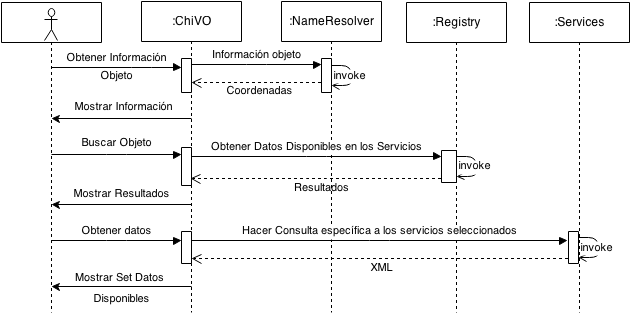
\includegraphics[width=0.7\textwidth]{images/secuencia.png}
    \caption{Diagrama de secuencia entre Usuario y ChiVO}
    \label{fig:secuencia}
\end{figure*}

La arquitectura de software de ChiVO está basada en el uso de protocolos y estándares de
IVOA. Estos protocolos y estándares están agrupados en capas, de las cuales
destacamos la capa de aplicación y la de datos (ver Figura~\ref{fig:ivoarch}),
ya que sus estándares básicos definen la operación mínima que un VO debe
realizar. A continuación, se detallan los elementos que ChiVO ha implementado
en estas capas.
\begin{figure}[ht]
    \centering
    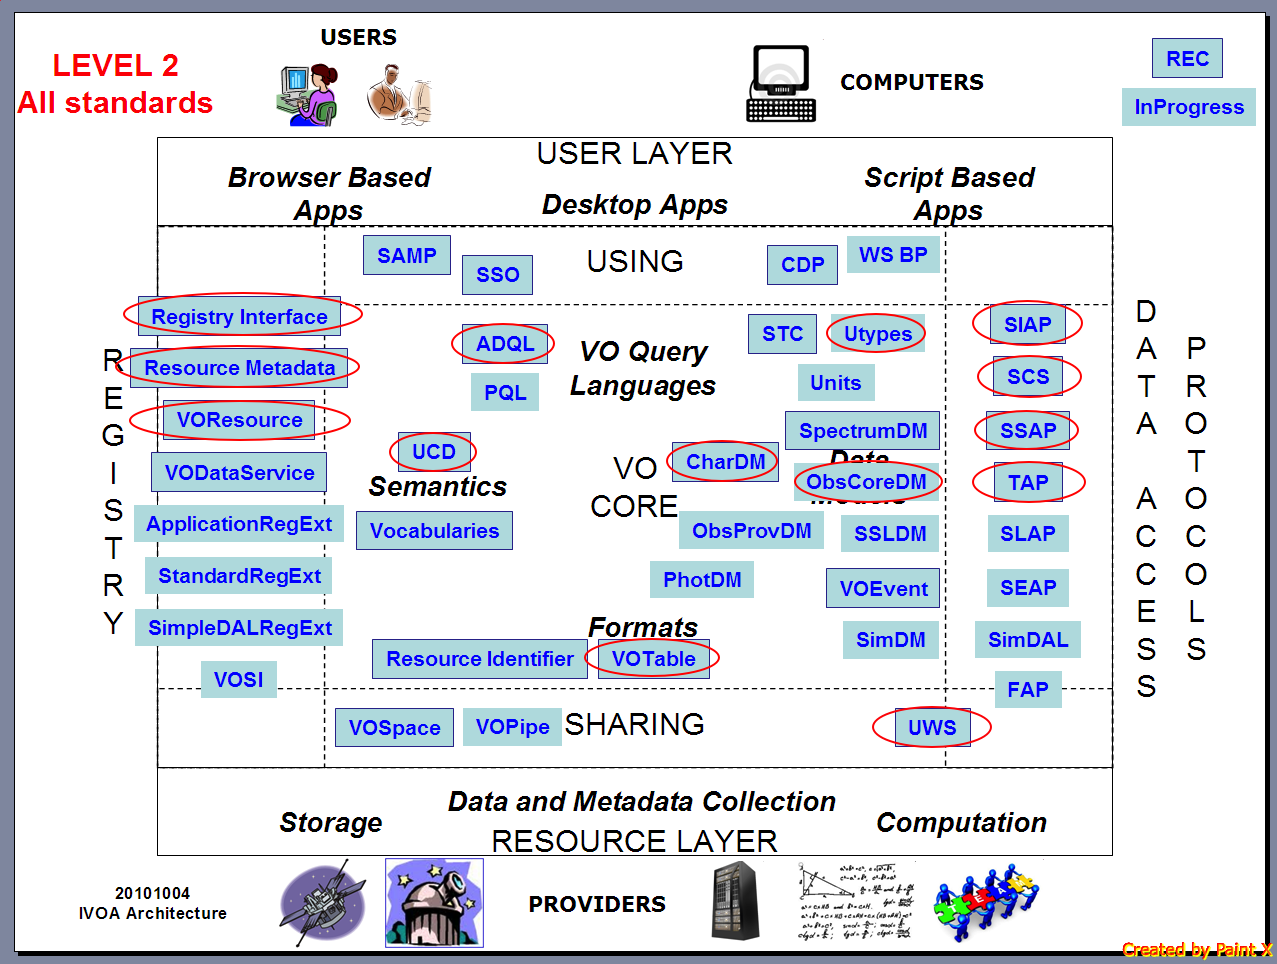
\includegraphics[width=0.45\textwidth]{images/arquitectura_2.png}
    \caption{Arquitectura de IVOA con los Protocolos y Estándares usados}
    \label{fig:ivoarch}
\end{figure}

\begin{description}
    \item[Capa Aplicación:] \hfill \\
        Un Servicio Web compatible con VO necesita al menos un \emph{Table Access
        Protocol} para acceder al modelo de datos de ChiVO usando el
        \emph{Astronomical Data Query Language}.
        Además, para el cumplimiento de los requerimientos del sistema,
        actualmente se ha implementado
        el protocolo para realizar búsquedas cónicas \emph{Simple Cone Search}, el protocolo para realizar acceder a datos
        espectrales \emph{Simple Spectral Access} y el protocolo de
        acceso a imágenes \emph{Simple Image Access}.

    \item[Capa de datos:] \hfill \\
        En esta capa se requiere la configuración de la base de datos relacional con
        un modelo de datos recomendado por IVOA llamado \emph{Observation Core Data
        Model}. Este modelo de datos permite que los VO sean interoperables,
        ya que definen una cantidad mínima de atributos en las tablas con cierto
        nombre y tipo de dato, de forma que acceder a diferentes servicios mediante
        \emph{TAP + Obscore} es estándar.
        Además el formato de transferencia de información (metadata) es con el
        formato estándar \emph{XML VOTable}.
\end{description}

\subsection{Capa de abstracción: Clientes}

Dento del diagrama de secuencia, el Frontend es el VO-Client, es decir, está a cargo
de generar la interacción entre los usuarios y los demás elementos dentro del
sistema.

Actualmente se generó un frontend en RoR que permite interactuar con:

\begin{description}
    \item[Resolver nombres]:\hfill \\
        a partir de un nombre (String) retorna la posición de un objeto en
        coordenadas celestiales usando el servicio SESAME de Astrogrid.
    \item[Registro]: \hfill \\
        busca servicios dentro del endpoint, y luego según lo que necesite el
        usuario elige sobre cuales trabajar para hacer consultas.
    \item[Servicios]: \hfill \\
        consulta a diferentes servicios web que proveen datos mediante cierto
        protocolo y unifica los resultados en un XML VOTable para ser desplegados
        en forma ordenada usando una biblioteca de javascript VOView.
\end{description}

\subsection{Capa de abstracción: Aplicaciones}

El Endpoint está a cargo de generar una interacción transparente entre los clientes
de VO y los posibles recursos que se configuren.
En este caso el Endpoint genera una interfaz para los servicios configurados por el
Backend y los disponibles a través del registro de VO-Paris.
VO-Paris posee una Web API en REST que permite consultar por recursos y retorna un
archivo JSON con resultados.

\subsection{Capa de abstracción: Datos}

Actualmente ALMA le facilita a ChiVO datos públicos, los cuales incluyen ASDM,
Measurement \cite{petry2012analysing}, FITS \cite{wells1981fits}, de los cuales es
necesario extraer los metadatos del ObsCoreDM para ser ingresados a la base de 
datos \ref{fig:metadata}.

\begin{figure}[h!t]
    \centering
    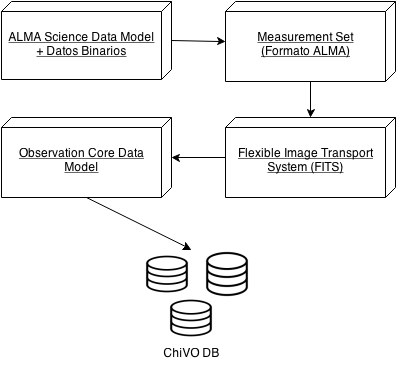
\includegraphics[width=0.45\textwidth]{images/metadata.png}
    \caption{Proceso transformación desde Frontend de ALMA hasta la base de datos
             de ChiVO}
    \label{fig:metadata}
\end{figure}

El procedimiento se hace a través de un programa, el cual usando el framework de
backend DaCHS, permite configurar recursos y servicios mediante
archivos de configuración Resource Descriptor \cite{dachsorguide}.
Una vez creadas las entradas en la base de datos y configurados los servicios SCS,
SSAP, SIAP, TAP se pueden acceder mediante las consultas definidas en cada
protocolo.


\section{Conclusiones y trabajo futuro}

El observatorio virtual es un \textit{framework} que le permite a los astrónomos y
comunidad en general buscar en múltiples servidores de datos de forma
transparente, pero un foco de mayor interés para la comunidad informática es
que guía la construcción de un sistema robusto a partir de tecnologías,
estándares y protocolos unificados. Esto enmarcado en su arquitectura orientada
a la intercomunicación mediante 3 capas: usuarios, intermedia (\textit{virtual
observatory}) y de recursos, y que gracias a la especificación de cada una,
están formalizados los formatos de representación de datos y los métodos por
los cuales se puede acceder a los mismos.

En el mundo hay 19 observatorios virtuales miembros de IVOA, y próximamente
Chile se unirá a esta organización mediante el Chilean Virtual Observatory, una
iniciativa en colaboración con 5 Universidades Chilenas, ALMA y REUNA.
Inicialmente el proyecto está centrado en capturar los requerimientos de los
astrónomos para una plataforma de este tipo y también en ver el modo de cómo
modelar los datos provenientes de ALMA de tal manera que sean útiles y
accesibles para la comunidad en general. Paralelamente se está haciendo un
estudio acabado de la arquitectura que plantea IVOA para usar y respetar
sus estándares de desarrollo y así asegurar la interoperabilidad de ChiVO
con los otros VOs del mundo.


\section*{Agradecimientos}
Este trabajo ha sido financiado parcialmente con el proyecto FONDEF D11I1060.

\section{Referencias}
\bibliographystyle{plain}
\bibliography{ccs}

\end{document}
